\documentclass{article}

\usepackage[utf8]{inputenc}
\usepackage[english]{babel}
\usepackage{amsthm}
\usepackage{amsmath, bm}
\usepackage[dvipsnames]{xcolor}
\usepackage{graphicx}
\usepackage{subcaption}
\captionsetup[subfigure]{font={bf,small}, skip=1pt, margin=-0.7cm, singlelinecheck=false}
\usepackage{bbm}
\usepackage{comment} 
\usepackage{cite}
\usepackage[colorlinks=true, allcolors=blue]{hyperref}
\usepackage{listings}
\usepackage{algcompatible}
% OR \usepackage{algorithmic}
\usepackage{algorithm}
\renewcommand{\algorithmicrequire}{\textbf{Input:}}
\renewcommand{\algorithmicensure}{\textbf{Output:}}
\usepackage{booktabs}
\newcommand{\bftab}{\fontseries{b}\selectfont}
\newcommand{\code}{\texttt}
\theoremstyle{definition}
\newtheorem*{remark}{Remark}
\newtheorem{definition}{Definition}

\usepackage[skip=10pt plus1pt]{parskip}
\usepackage{setspace}
\onehalfspacing
\usepackage[letterpaper,top=2cm,bottom=2cm,left=3cm,right=3cm,marginparwidth=1.75cm]{geometry}


\title{Beyond forecast leaderboards: Measuring individual model importance based on contribution to probabilistic ensemble accuracy}
\author{Minsu Kim, Evan L. Ray, Nicholas G. Reich}
\date{}


\usepackage{Sweave}
\begin{document}
\Sconcordance{concordance:manuscript.tex:manuscript.Rnw:1 32 1 1 0 3 1 1 10 14 1 1 58 %
1 3 16 1 1 19 1 3 14 1 1 22 1 2 11 1}

\maketitle



\begin{abstract}
Ensemble forecasting is generally recognized for its ability to outperform individual standalone models in infectious disease forecasting and is therefore considered a robust option for public health decision making and policy planning. The US COVID-19 Forecast Hub has produced a probabilistic ensemble forecast model of COVID-19 cases, hospitalizations, and deaths in the United States based on forecasts from individual models developed by more than 90 different research groups. As the Forecast Hub served as the official short-term forecast of the US Centers for Disease Control and Prevention, it is important to understand the relative importance and contributions of individual models to creating a highly accurate forecast combination. 
In this work, we propose two practical methods for evaluating the contribution of individual component models. 
One method uses a leave-one-model-out algorithm when building an ensemble and the other, based on the Shapley value in game theory, considers ensemble models constructed from all possible subsets of individual models. 
We aim to identify and evaluate methods for measuring the contributions of individual component models to ensemble accuracy. We explore how these metrics are related to the weighted interval score (WIS), a commonly used proper scoring rule for quantile forecasts, and illustrate how these methods provide distinct perspectives when evaluating how much value a component model adds to a probabilistic ensemble model in the presence of other models. Our results show that the most accurate model according to WIS does not always add the most value to the ensemble. This indicates that our proposed methods can be used to capture the contribution of individual models to a more accurate ensemble model, which is difficult to ascertain from standard accuracy metrics alone. This study offers valuable insights into understanding individual forecasting models’ unique features and their roles in contributing to an ensemble model for a specific prediction task.
    
\end{abstract}

\section{Introduction}

\begin{figure}[b!]
\centering

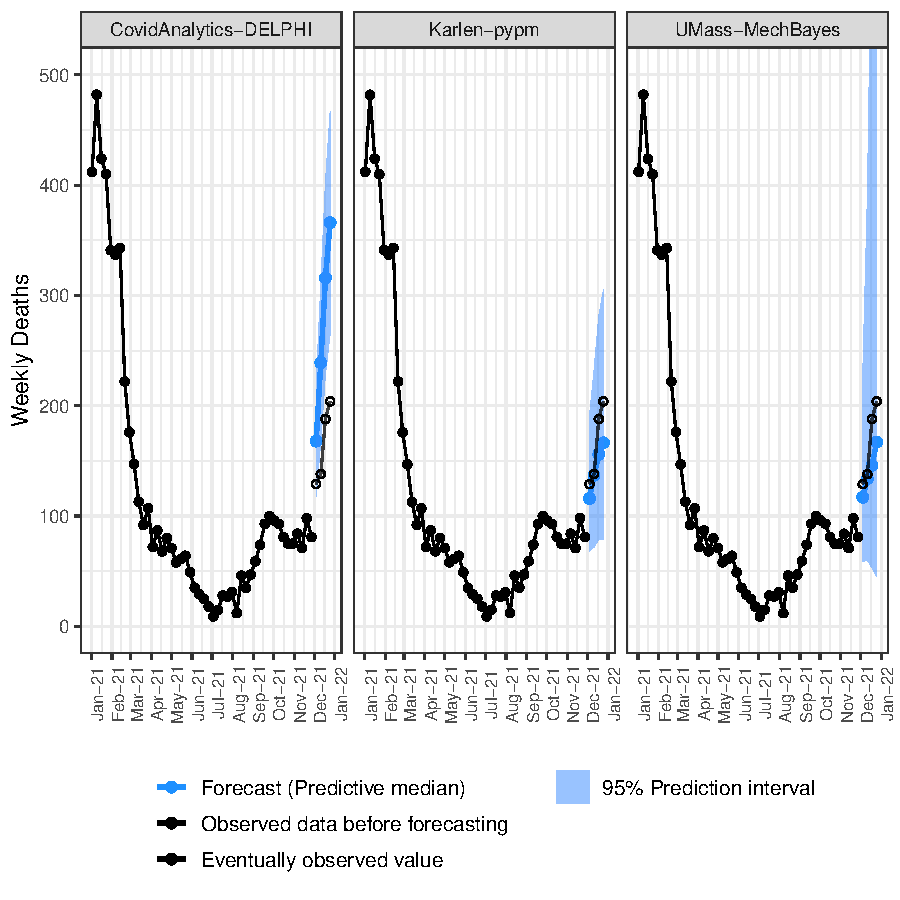
\includegraphics{manuscript-fig1.motivation-example}

\caption{Forecasts of COVID-19 incident deaths at 1- through 4-week horizons in Massachusetts made on November 27, 2021 by three models. Black dots show historical data available as of November 28. Blue dots indicate predictive medians and the shaded bands represent 95\% prediction intervals. The open black circles are observations not available when the forecast was made. The 95\% prediction intervals of the UMass-MechBayes model (truncated here for better visibility of the observed data) extend up to 671 and 1110 for the 3-week and 4-week ahead horizons, respectively. }
\label{fig:forecasts-example}
\end{figure}

\newpage
\section{Methods}\label{sec:methods}

\newpage
\section{Results}\label{sec:result}

\subsection{Application of the model importance metrics to forecast data from the US COVID-19 Forecast Hub}\label{subsec:application}

\subsubsection{Case study: Relationship between importance score and WIS with data for deaths in Massachusetts in 2021}

\begin{figure}[b!]
\centering
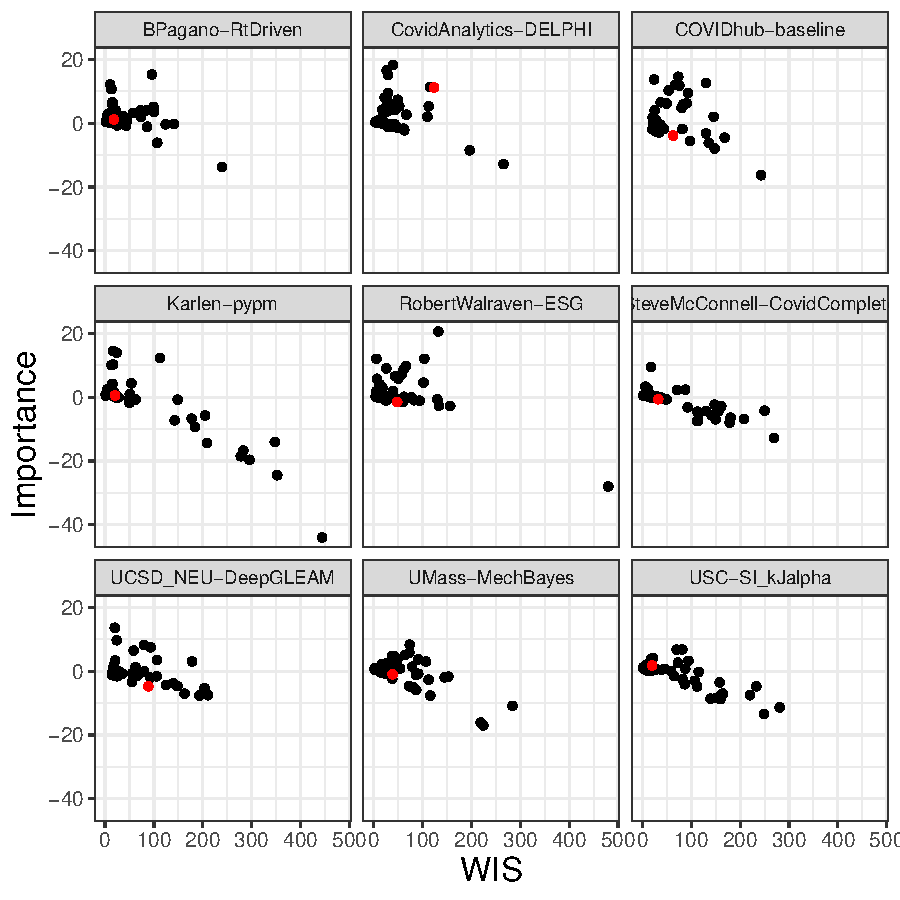
\includegraphics{manuscript-fig2.importance-vs-wis-by-model}

\caption{Model importance versus WIS by model for all weeks in 2021. Each point represents a pair of WIS and importance score evaluated at a certain week, and each panel contains 52 points accordingly. Red dots represent WIS and importance score pairs evaluated on December 25, 2021. The importance of an individual model as an ensemble member tends to be inversely correlated with that model's overall prediction accuracy.}
\label{fig:scatterplot-wis_imp2021}
\end{figure}


\begin{figure}
\centering
\begin{subfigure}{\textwidth}
	\subcaption{}
\includegraphics{manuscript-fig3-1.wis_imp20211225}

\label{fig:plot-wis_imp20211225}
\end{subfigure}\par
\begin{subfigure}{\textwidth}
	\subcaption{}
	\includegraphics[scale=0.55]{manuscript-fig3-2.95PIs.pdf}
		\label{fig:PIs2021}
\end{subfigure}
\caption{(\subref{fig:PIs2021}) 95\% Prediction intervals (PIs) of individual forecasts (top) and ensemble forecasts built excluding a single model (bottom) on target end date 2021-12-25. For example, the lines on the far left indicate PI for the CovidAnalytics-DELPHI model on the top panel and PI for the ensemble created without the CovidAnalytics-DELPHI model on the bottom panel. Ensemble.ALL represents an ensemble model built on all nine individual models. In each PI, the  end points indicate 0.025 and 0.975 quantiles and the mid-point represents the 0.5 quantile (predictive median). The horizontal dashed lines represent the eventual observation. The ensemble without CovidAnalytics-DELPHI is the only ensemble model with a point estimate below 150. The ensemble without UMass-MechBayes has the lowest dispersion
among the ensemble models. (\subref{fig:plot-wis_imp20211225}) Model importance of each model versus WIS on target end date 2021-12-25. CovidAnalytics-DELPHI is the most important and also the least accurate by WIS.}
\label{fig:20211225}
\end{figure}



\newpage
\subsubsection{Differences in importance scores measured by different algorithms and ensemble methods}

% latex table generated in R 4.3.2 by xtable 1.8-4 package
% Tue Feb 27 09:30:24 2024
\begin{table}[ht]
\centering
\begin{tabular}{|ccc|}
  \hline
Model & Submission rate (\%) & Number of predictions (total:21800) \\ 
  \hline
BPagano-RtDriven & 100.0 & 21800 \\ 
  COVIDhub-baseline & 100.0 & 21800 \\ 
  CU-select & 96.3 & 21000 \\ 
  USC-SI\_kJalpha & 95.9 & 20900 \\ 
  GT-DeepCOVID & 95.1 & 20724 \\ 
  MOBS-GLEAM\_COVID & 94.5 & 20596 \\ 
  UCSD\_NEU-DeepGLEAM & 94.5 & 20596 \\ 
  Karlen-pypm & 93.6 & 20400 \\ 
  PSI-DRAFT & 91.7 & 19988 \\ 
  RobertWalraven-ESG & 91.7 & 19992 \\ 
   \hline
\end{tabular}
\caption{Submission rates (rounded to one decimal place) and the number of individual forecasts made by 10 models for the US 50 states and 1-4 horizons from November 2020 to November 2022 (109 weeks).} 
\end{table}


\begin{figure}[h!]
\centering
\includegraphics{manuscript-fig4.corr-NAworst}

\caption{Relationship between summary metrics computed across the entire evaluation period. One black dot corresponds to one model, with the position representing the average scores across the entire evaluation period for the metrics corresponding to the row and column of the plot matrix.}
\label{fig:corr-NAworst} 
\end{figure}


% latex table generated in R 4.3.2 by xtable 1.8-4 package
% Tue Feb 27 09:30:27 2024
\begin{table}[ht]
\centering
\begin{tabular}{|rccccccc|}
  \hline
Model &  WIS & relWIS & Rank & $\Phi^{\text{lasomo}}_{\text{eq}}$ & $\Phi^{\text{lasomo}}_{\text{wt}}$ & $\Phi^{\text{lomo}}_{\text{eq}}$ & $\Phi^{\text{lomo}}_{\text{wt}}$ \\ 
  \hline
BPagano-RtDriven & 40.2 & 0.77 & 0.59 & 2.81 & 2.59 & 0.71 & 0.36 \\ 
  Karlen-pypm & 41.2 & 0.79 & 0.59 & 3.11 & 3.63 & 0.92 & 1.21 \\ 
  GT-DeepCOVID & 42.8 & 0.82 & 0.54 & 1.87 & 1.93 & 0.17 & -0.03 \\ 
  MOBS-GLEAM\_COVID & 45.8 & 0.88 & 0.52 & 1.06 & 1.32 & -0.21 & -0.11 \\ 
  CU-select & 47.3 & 0.91 & 0.49 & 1.64 & 1.41 & 0.24 & 0.13 \\ 
  RobertWalraven-ESG & 49.8 & 0.96 & 0.49 & 0.94 & 1.11 & -0.09 & -0.15 \\ 
  USC-SI\_kJalpha & 51.7 & 0.99 & 0.49 & 1.23 & 0.85 & 0.21 & -0.49 \\ 
  COVIDhub-baseline & 52.1 & 1.00 & 0.42 & 0.10 & 0.62 & -0.62 & -0.14 \\ 
  UCSD\_NEU-DeepGLEAM & 52.6 & 1.01 & 0.26 & -0.13 & 0.65 & -0.70 & -0.29 \\ 
  PSI-DRAFT & 71.7 & 1.38 & 0.39 & -1.94 & -0.94 & -1.00 & -0.95 \\ 
   \hline
\end{tabular}
\caption{Summary of WIS, relative WIS compared to the COVIDhub-baseline, standardized rank score, importance scores ($\Phi$), sorted by mean WIS. All scores were averaged across all forecast dates, locations, and horizons. In the importance score notation ($\Phi$), the superscript indicates the algorithm method, and the subscript indicates the ensemble method used. For example, $\Phi^{\text{lomo}}_{\text{wt}}$ represents the mean important score based on leave one model out algorithm with weighted (trained) ensemble and $\Phi^{\text{lasomo}}_{\text{eq}}$ represents the mean important score based on leave all subsets of models out algorithm with equally weighted (untrained) ensemble.  The best value in each column is highlighted in bold.} 
\end{table}

\section{Simulation Studies} \label{simulation}

\subsection{Relationship between a component forecaster's bias and importance}


\begin{figure}[h!]
	\centering
\includegraphics{manuscript-fig5.simuplot-imp_bias}
	\caption{Importance of three forecasters by various biases of forecaster 3. $F_{1,t} = \text{N}(-1, 1)$, $F_{2,t} = \text{N}(-0.5, 1)$, and $F_{3,t} = \text{N}(b, 1)$. Importance scores were calculated and averaged over 1000 replicates of the forecasting experiments conducted at each value of $b$, incremented by 0.05 from $-1$ to $3$. The results are displayed in different line patterns by model (dashed line for forecaster 1, dash-dotted line for forecaster 2, and solid line for forecaster 3). }
	\label{fig:simuplot-imp_bias}
\end{figure}

\newpage
\subsection{Relationship between component forecaster dispersion and importance}


\begin{figure}[h!]
	\centering
\includegraphics{manuscript-fig6.simuplot-imp_dispersion}
	\caption{Importance of three forecasters as a function of dispersion of forecaster 3. $F_{1,t} = \text{N}(0, 0.5^2)$, $F_{2,t} = \text{N}(0, 0.7^2)$, and $F_{3,t} = \text{N}(0, s^2).$ Importance scores were calculated and averaged over 1000 replicates of the forecasting experiments conducted at each value of $s$, incremented by 0.05 from $0.1$ to $3$. The results are displayed in different line patterns by model (dashed line for forecaster 1, dash-dotted line for forecaster 2, and solid line for forecaster 3).}
	\label{fig:simuplot-imp_dispersion}
\end{figure}



\end{document}
